\chapter{Chapter \ref{ChapterPreTrip} Preliminary Survey}
\label{AppendixD}

The following sections show screenshots of the preliminary survey given to participants in the within-subject study described in Chapter \ref{ChapterPreTrip}. The preliminary survey in Chapter \ref{ChapterNavigo} is derived from this with only a few modifications.

\section{Project Description and Consent}
This section of the survey gives a brief description of the study, as well as the benefits and expectations for the participant. At the end is the consent and screener questions to make sure that the participant fits the inclusion criteria. 
\begin{figure}[t]
  \centering
  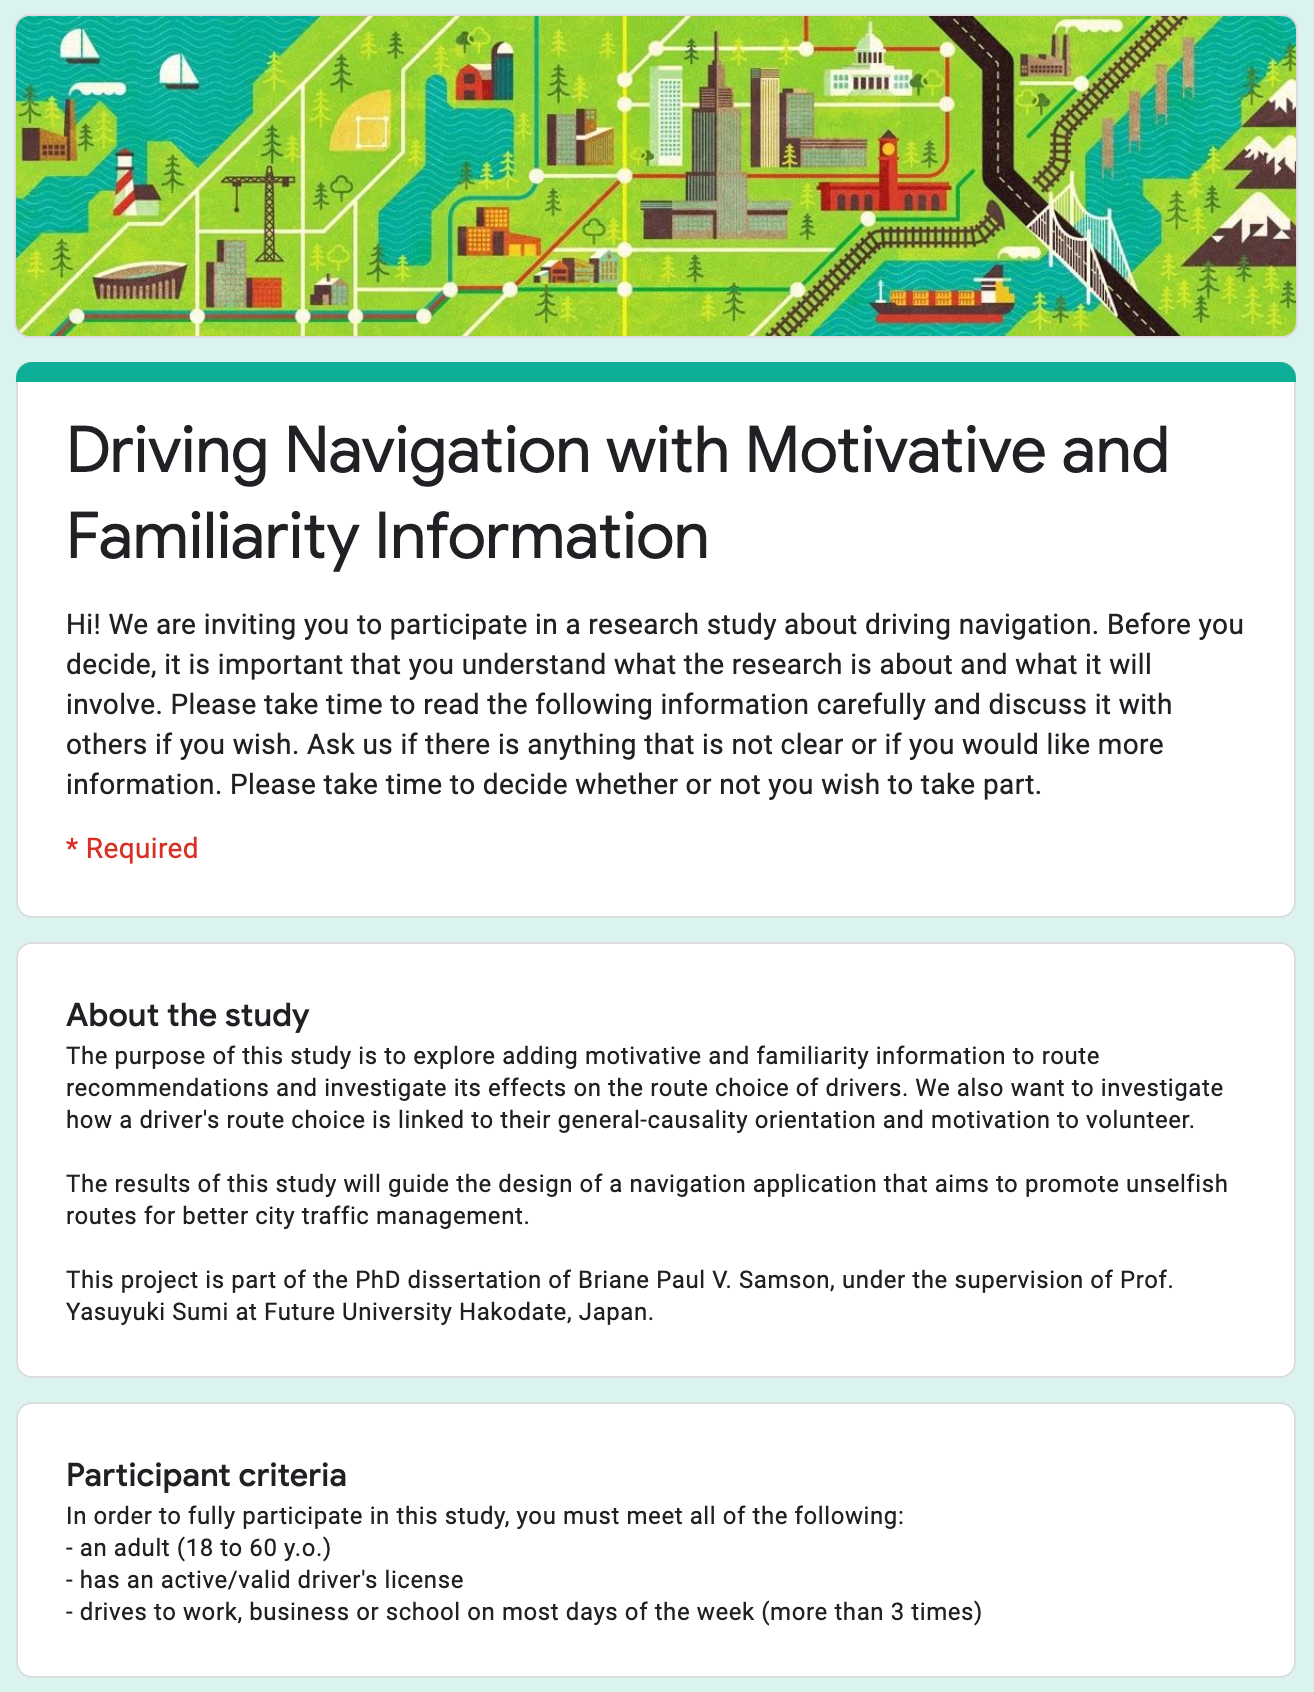
\includegraphics[scale=0.6]{figures/d-info1.png}
\end{figure}

\begin{figure}[h]
  \centering
  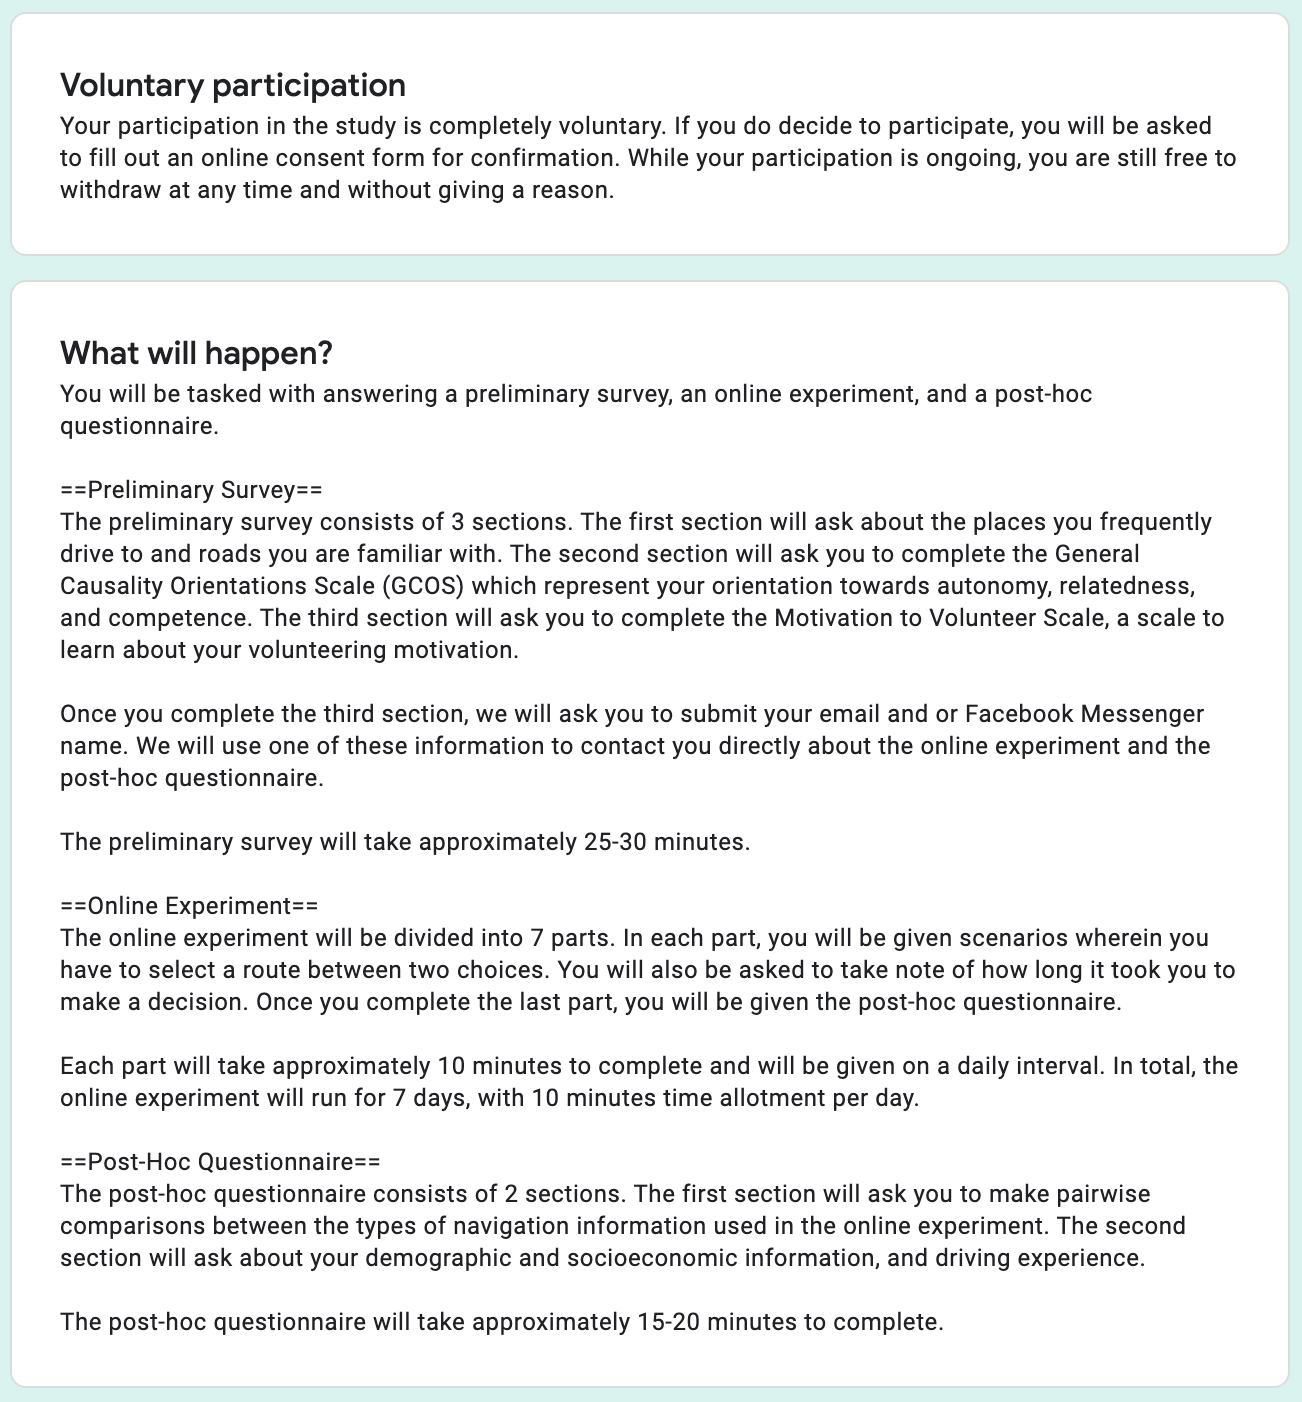
\includegraphics[scale=0.6]{figures/d-info2.png}
\end{figure}

\begin{figure}[h]
  \centering
  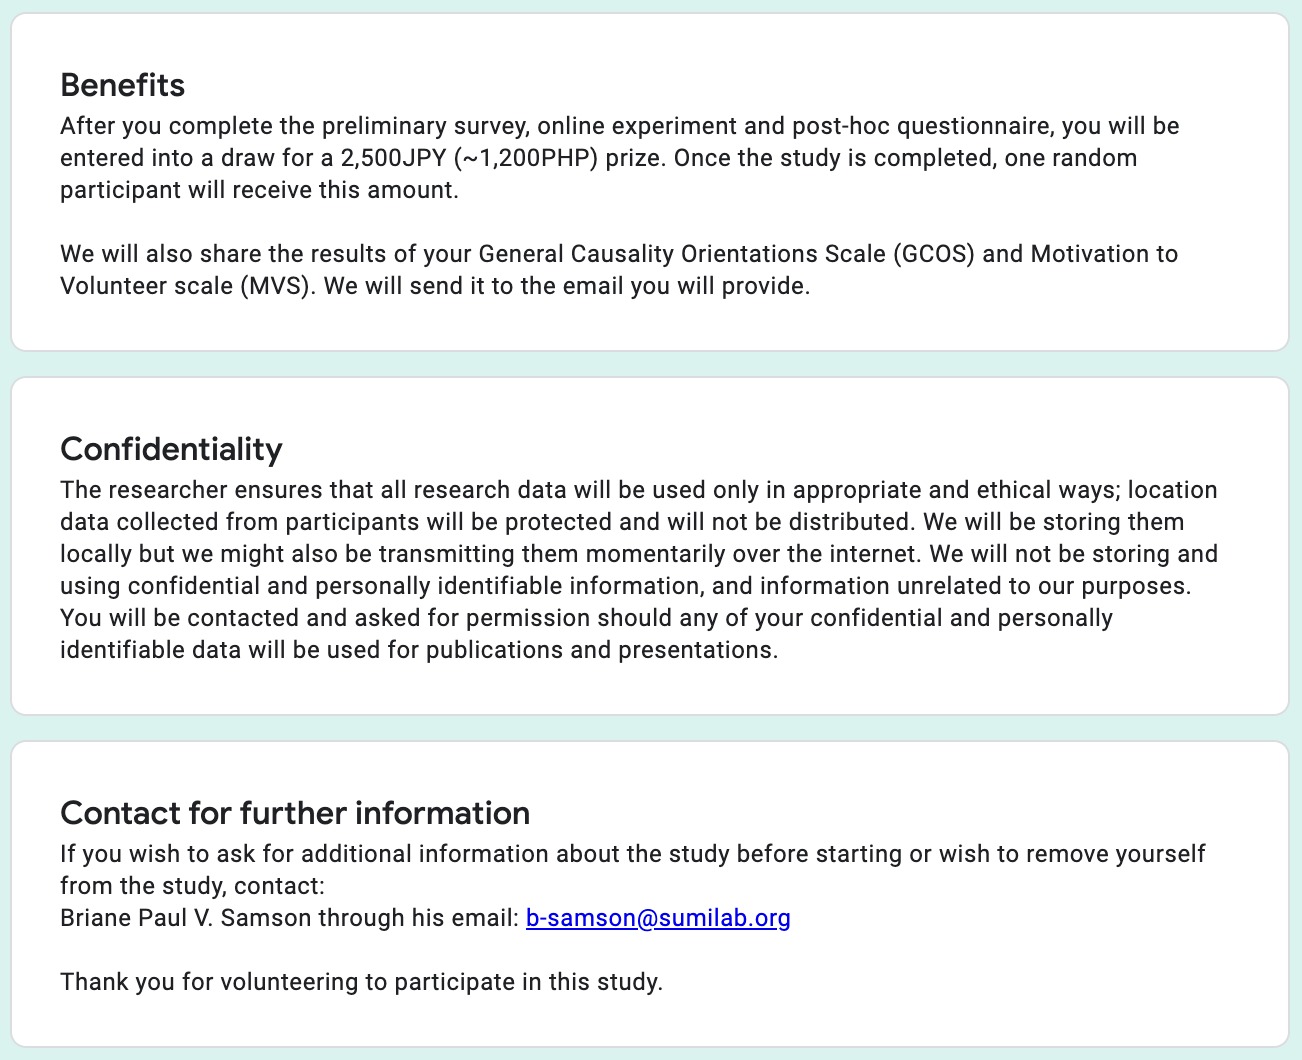
\includegraphics[scale=0.6]{figures/d-info3.png}
\end{figure}

\begin{figure}[h]
  \centering
  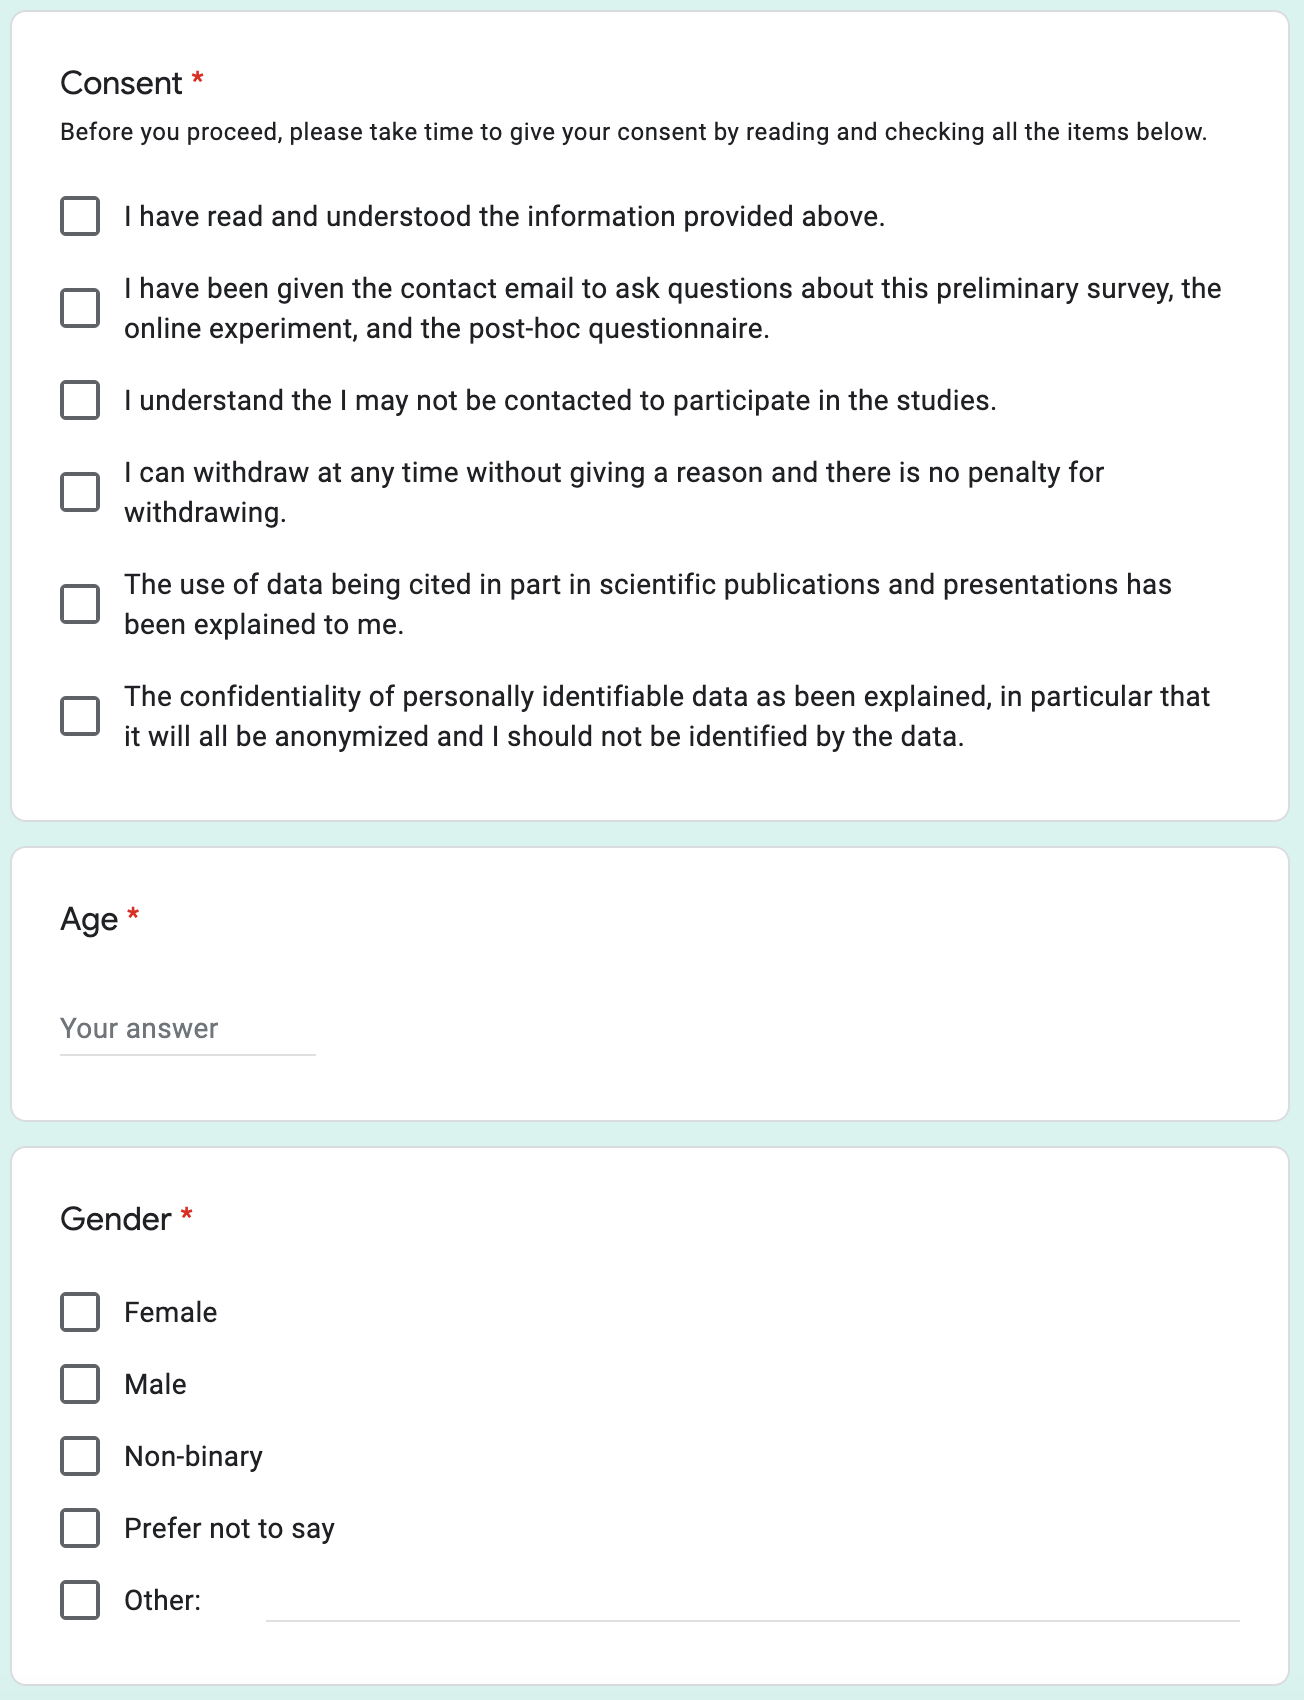
\includegraphics[scale=0.6]{figures/d-info4.png}
\end{figure}

\begin{figure}[h]
  \centering
  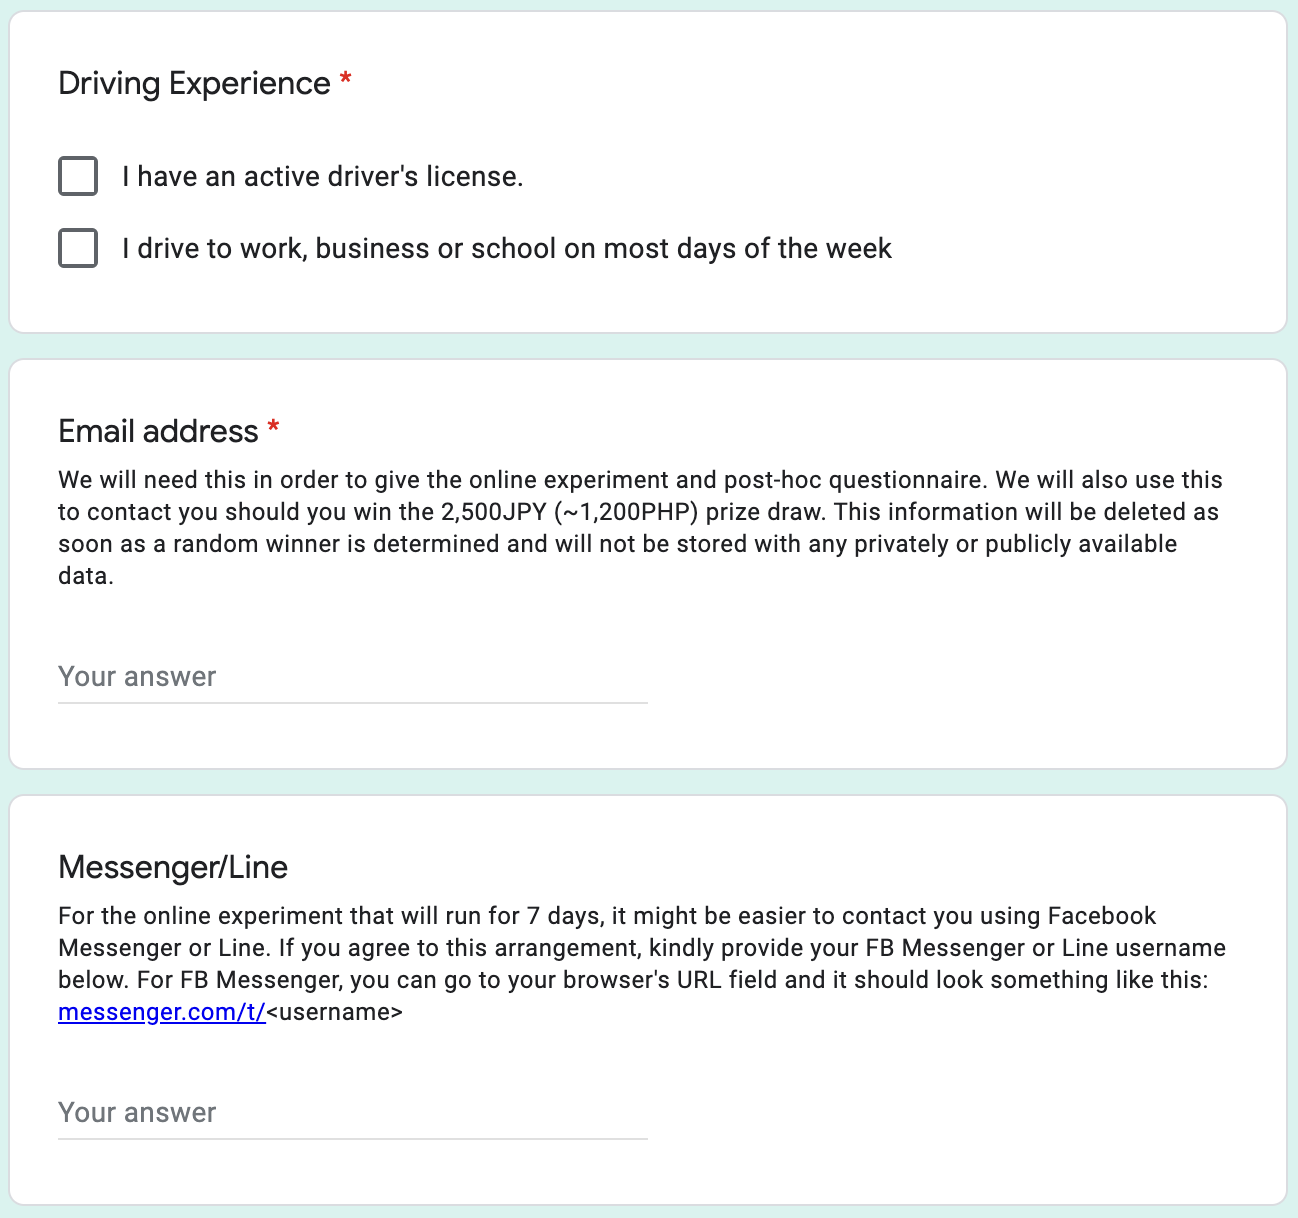
\includegraphics[scale=0.6]{figures/d-info5.png}
\end{figure}
\clearpage

\section{Travel Information}
This section asks for the home and work/school locations of the participants. It also asks for two frequently visited locations and names of familiar roads. Lastly, it asks how often they switch between their regular and alternative routes before the pandemic. All information gathered here will be kept confidential and will be deleted after the study. 
\begin{figure}[h]
  \centering
  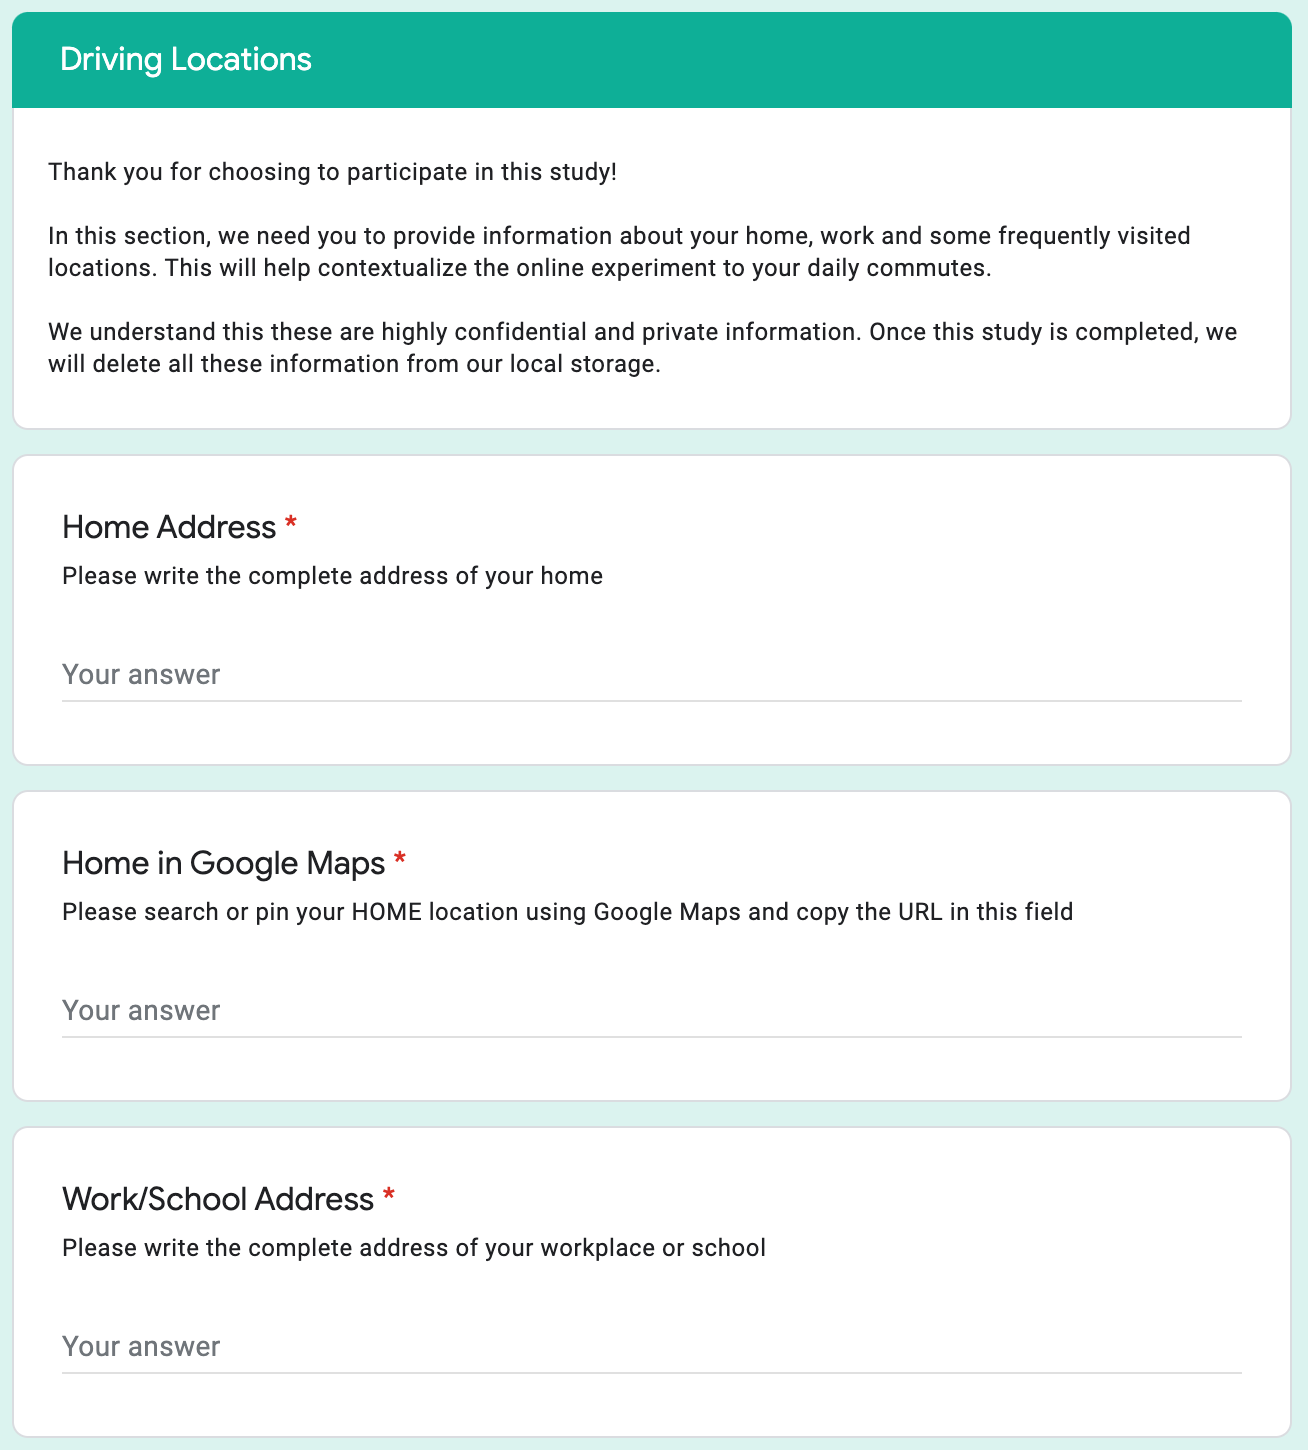
\includegraphics[scale=0.6]{figures/d-travel1.png}
\end{figure}

\begin{figure}[h]
  \centering
  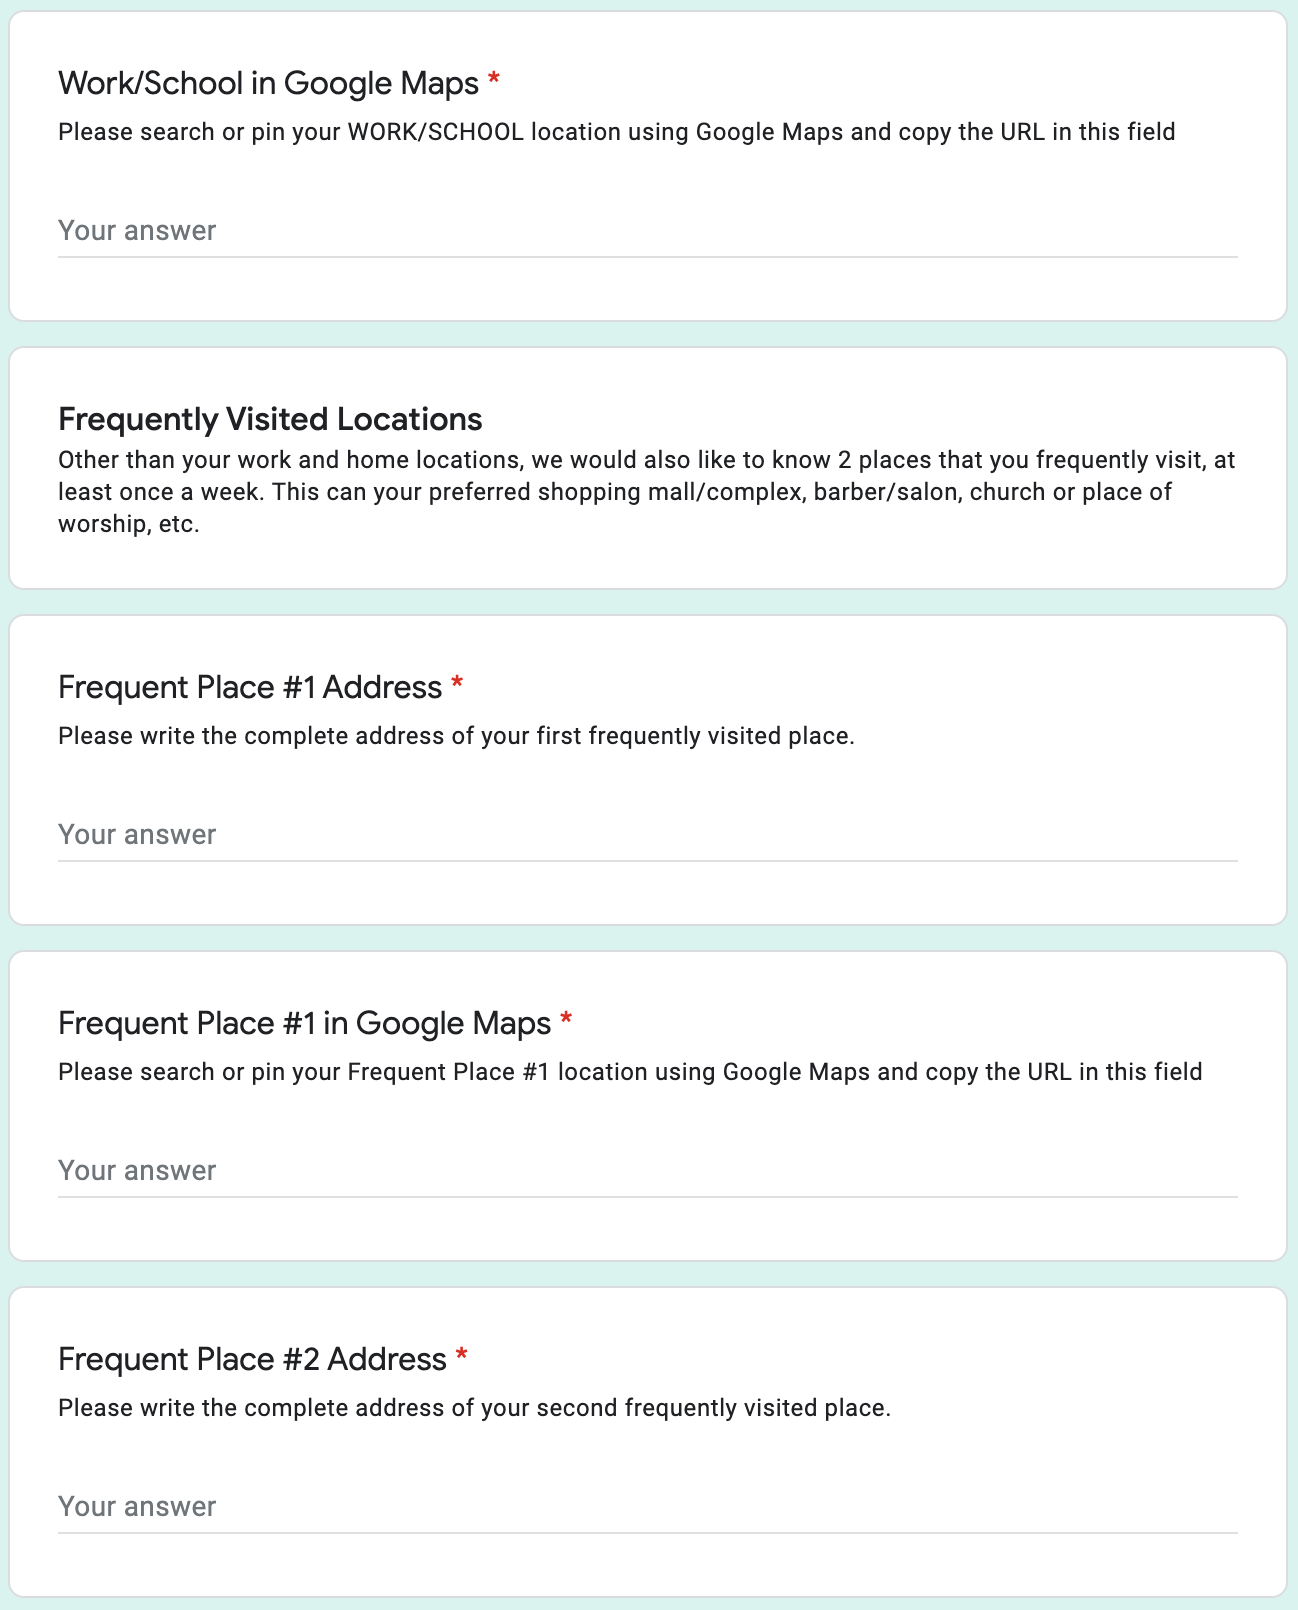
\includegraphics[scale=0.6]{figures/d-travel2.png}
\end{figure}

\begin{figure}[h]
  \centering
  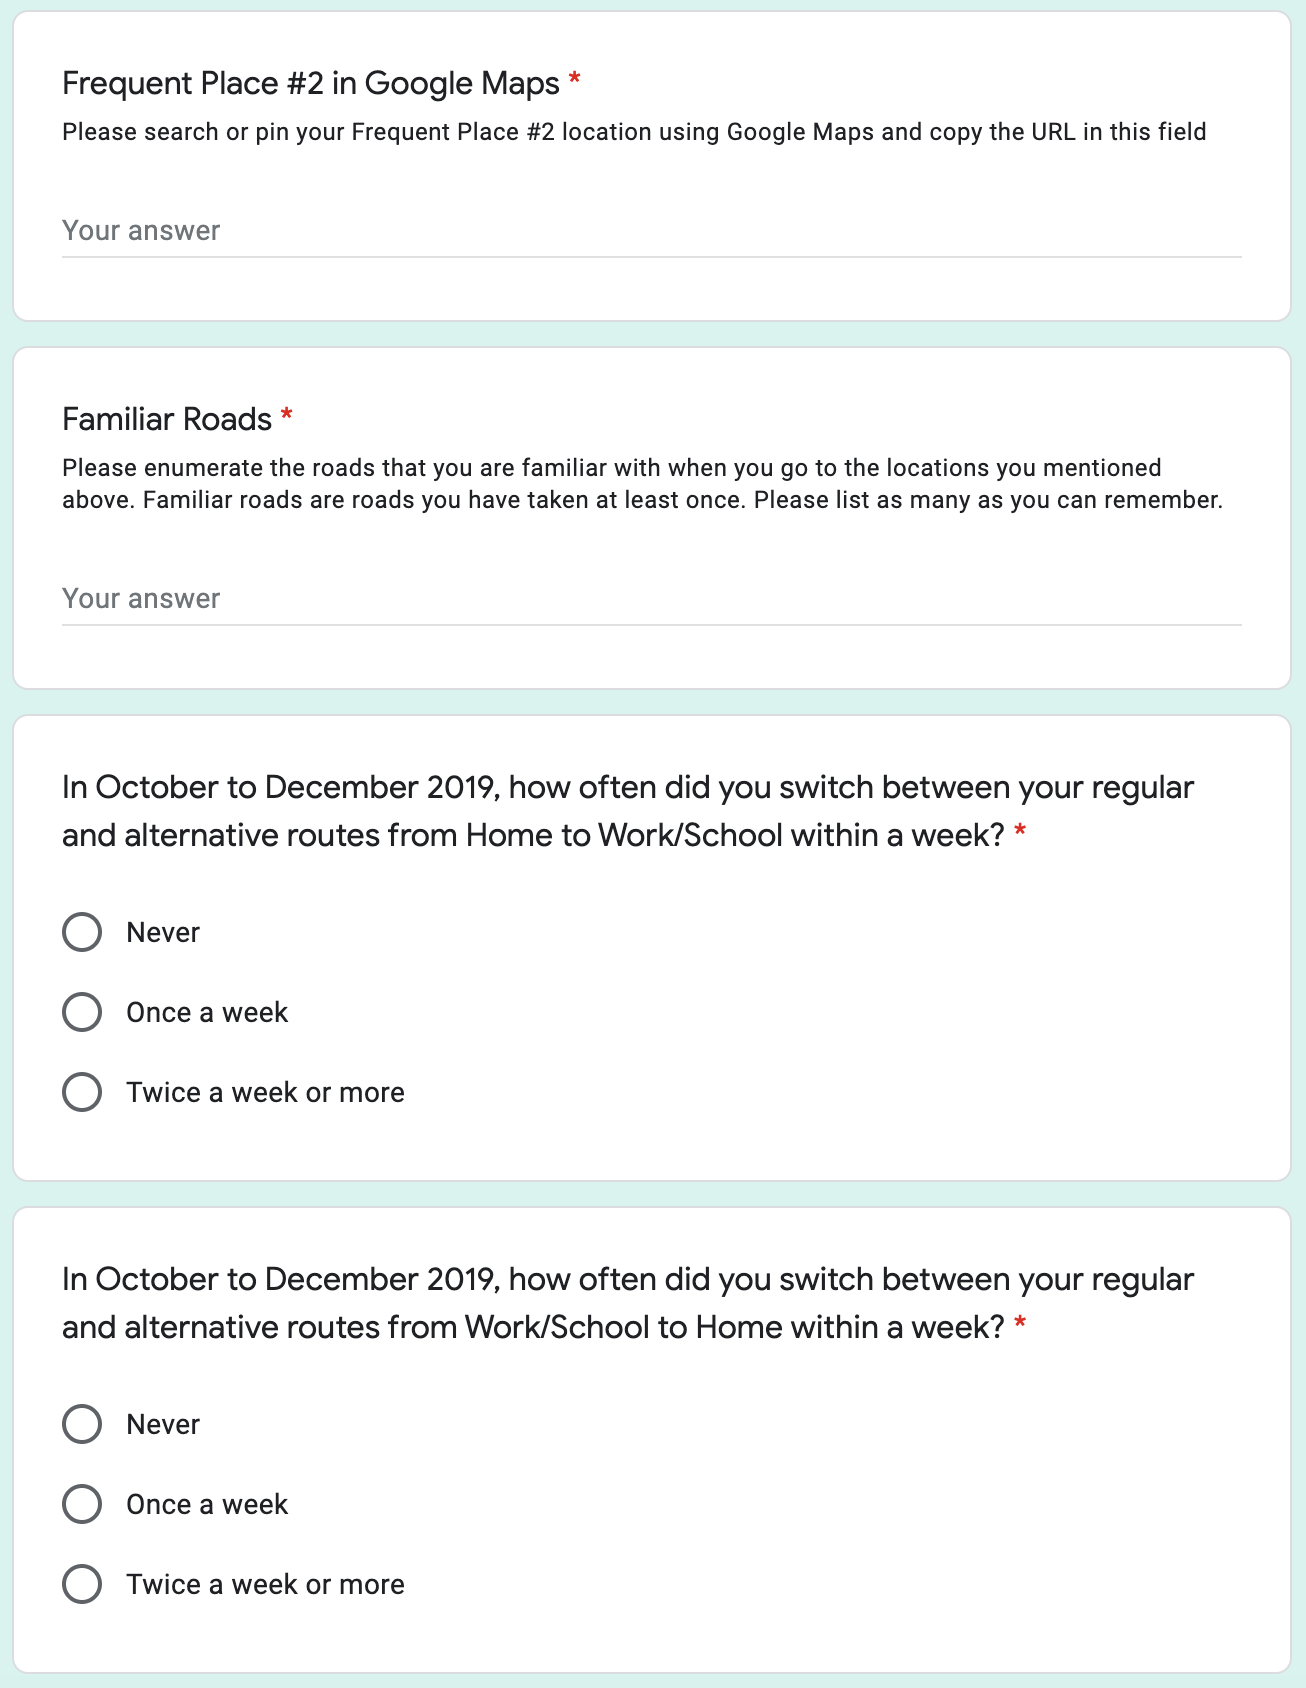
\includegraphics[scale=0.6]{figures/d-travel3.png}
\end{figure}
\clearpage

\section{General Causality Orientation Survey}
\begin{figure}[h]
  \centering
  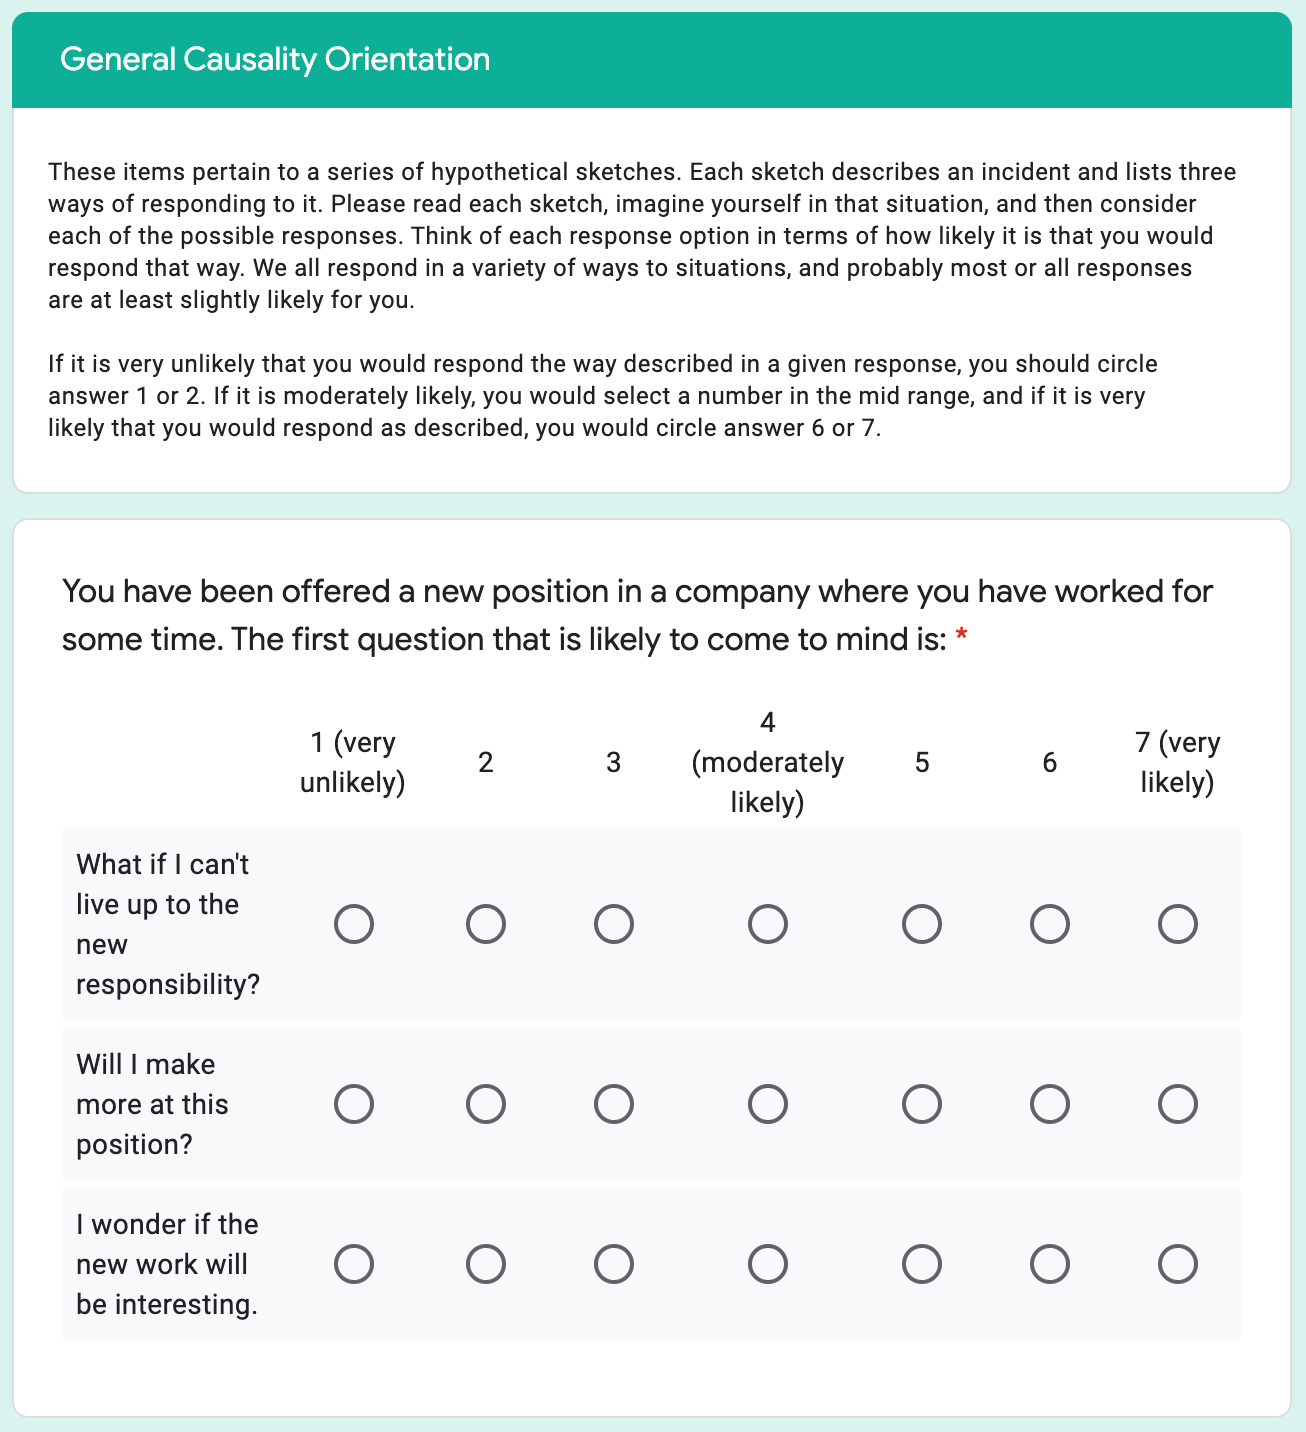
\includegraphics[scale=0.6]{figures/d-gcos.png}
\end{figure}
The General Causality Orientation survey is derived from Self-Determination Theory\cite{Deci1985GCOS} which assesses the strength of an individual's motivational orientations. The survey presents a series of hypothetical sketches that requires participants to imagine themselves in a situation. For each sketch, they must answer how likely it is they think they would respond in a particular way. Each item are answerable with a Likert-type scale from 1 to 7, with 1 being very unlikely and 7 as very likely. The figure above shows how the survey looks in Google Forms. The following are the 12 vignettes shown to the participants.

\begin{enumerate}
    \item You have been offered a new position in a company where you have worked for some time. The first question that is likely to come to mind is:
    \begin{enumerate}
        \item What if I can't live up to the new responsibility?
        \item Will I make more at this position?
        \item I wonder if the new work will be interesting.
    \end{enumerate}
    \item You have a school-age daughter. On parents' night the teacher tells you that your daughter is doing poorly and doesn't seem involved in the work. You are likely to:
    \begin{enumerate}
        \item Talk it over with your daughter to understand further what the problem is.
        \item Scold her and hope she does better.
        \item Make sure she does the assignments, because she should be working harder.
    \end{enumerate}
    \item You had a job interview several weeks ago. In the mail you received a form letter which states that the position has been filled. It is likely that you might think:
    \begin{enumerate}
        \item It's not what you know, but who you know.
        \item I'm probably not good enough for the job.
        \item Somehow they didn't see my qualifications as matching their needs.
    \end{enumerate}
    \item You are a plant supervisor and have been charged with the task of allotting coffee breaks to three workers who cannot all break at once. You would likely handle this by:
    \begin{enumerate}
        \item Telling the three workers the situation and having them work with you on the schedule.
        \item Simply assigning times that each can break to avoid any problems.
        \item Find out from someone in authority what to do or do what was done in the past.
    \end{enumerate}
    \item A close (same-sex) friend of yours has been moody lately, and a couple of times has become very angry with you over "nothing." You might:
    \begin{enumerate}
        \item Share your observations with him/her and try to find out what is going on for him/her.
        \item Ignore it because there's not much you can do about it anyway.
        \item Tell him/her that you're willing to spend time together if and only if he/she makes more effort to control him/herself.
    \end{enumerate}
    \item You have just received the results of a test you took, and you discovered that you did very poorly. Your initial reaction is likely to be:
    \begin{enumerate}
        \item ``I can't do anything right,'' and feel sad.
        \item ``I wonder how it is I did so poorly,'' and feel disappointed.
        \item ``That stupid test doesn't show anything,'' and feel angry.
    \end{enumerate}
    \item You have been invited to a large party where you know very few people. As you look forward to the evening, you would likely expect that:
    \begin{enumerate}
        \item You'll try to fit in with whatever is happening in order to have a good time and not look bad.
        \item You'll find some people with whom you can relate.
        \item You'll probably feel somewhat isolated and unnoticed.
    \end{enumerate}
    \item You are asked to plan a picnic for yourself and your fellow employees. Your style for approaching this project could most likely be characterized as:
    \begin{enumerate}
        \item Take charge: that is, you would make most of the major decisions yourself.
        \item Follow precedent: you're not really up to the task so you'd do it the way it's been done before.
        \item Seek participation: get inputs from others who want to make them before you make the final plans.
    \end{enumerate}
    \item Recently a position opened up at your place of work that could have meant a promotion for you. However, a person you work with was offered the job rather than you. In evaluating the situation, you're likely to think:
    \begin{enumerate}
        \item You didn't really expect the job; you frequently get passed over.
        \item The other person probably "did the right things" politically to get the job.
        \item You would probably take a look at factors in your own performance that led you to be passed over.
    \end{enumerate}
    \item You are embarking on a new career. The most important consideration is likely to be:
    \begin{enumerate}
        \item Whether you can do the work without getting in over your head.
        \item How interested you are in that kind of work.
        \item Whether there are good possibilities for advancement.
    \end{enumerate}
    \item A woman who works for you has generally done an adequate job. However, for the past two weeks her work has not been up to par and she appears to be less actively interested in her work. Your reaction is likely to be:
    \begin{enumerate}
        \item Tell her that her work is below what is expected and that she should start working harder.
        \item Ask her about the problem and let her know you are available to help work it out.
        \item It's hard to know what to do to get her straightened out.
    \end{enumerate}
    \item Your company has promoted you to a position in a city far from your present location. As you think about the move you would probably:
    \begin{enumerate}
        \item Feel interested in the new challenge and a little nervous at the same time.
        \item Feel excited about the higher status and salary that is involved.
        \item Feel stressed and anxious about the upcoming changes.
    \end{enumerate}
\end{enumerate}

\section{Motivation to Volunteer Survey}
The Motivation to Volunteer Survey is intended to measure an individual's motivations for volunteering by measuring their different behavioral regulatory styles based on SDT. Each item is answerable with Likert-type scale from 1 to 5. The figure below shows how the survey looks in Google Forms. The following are the 24 vignettes shown to the participants with one attention check item.
\begin{figure}[h]
  \centering
  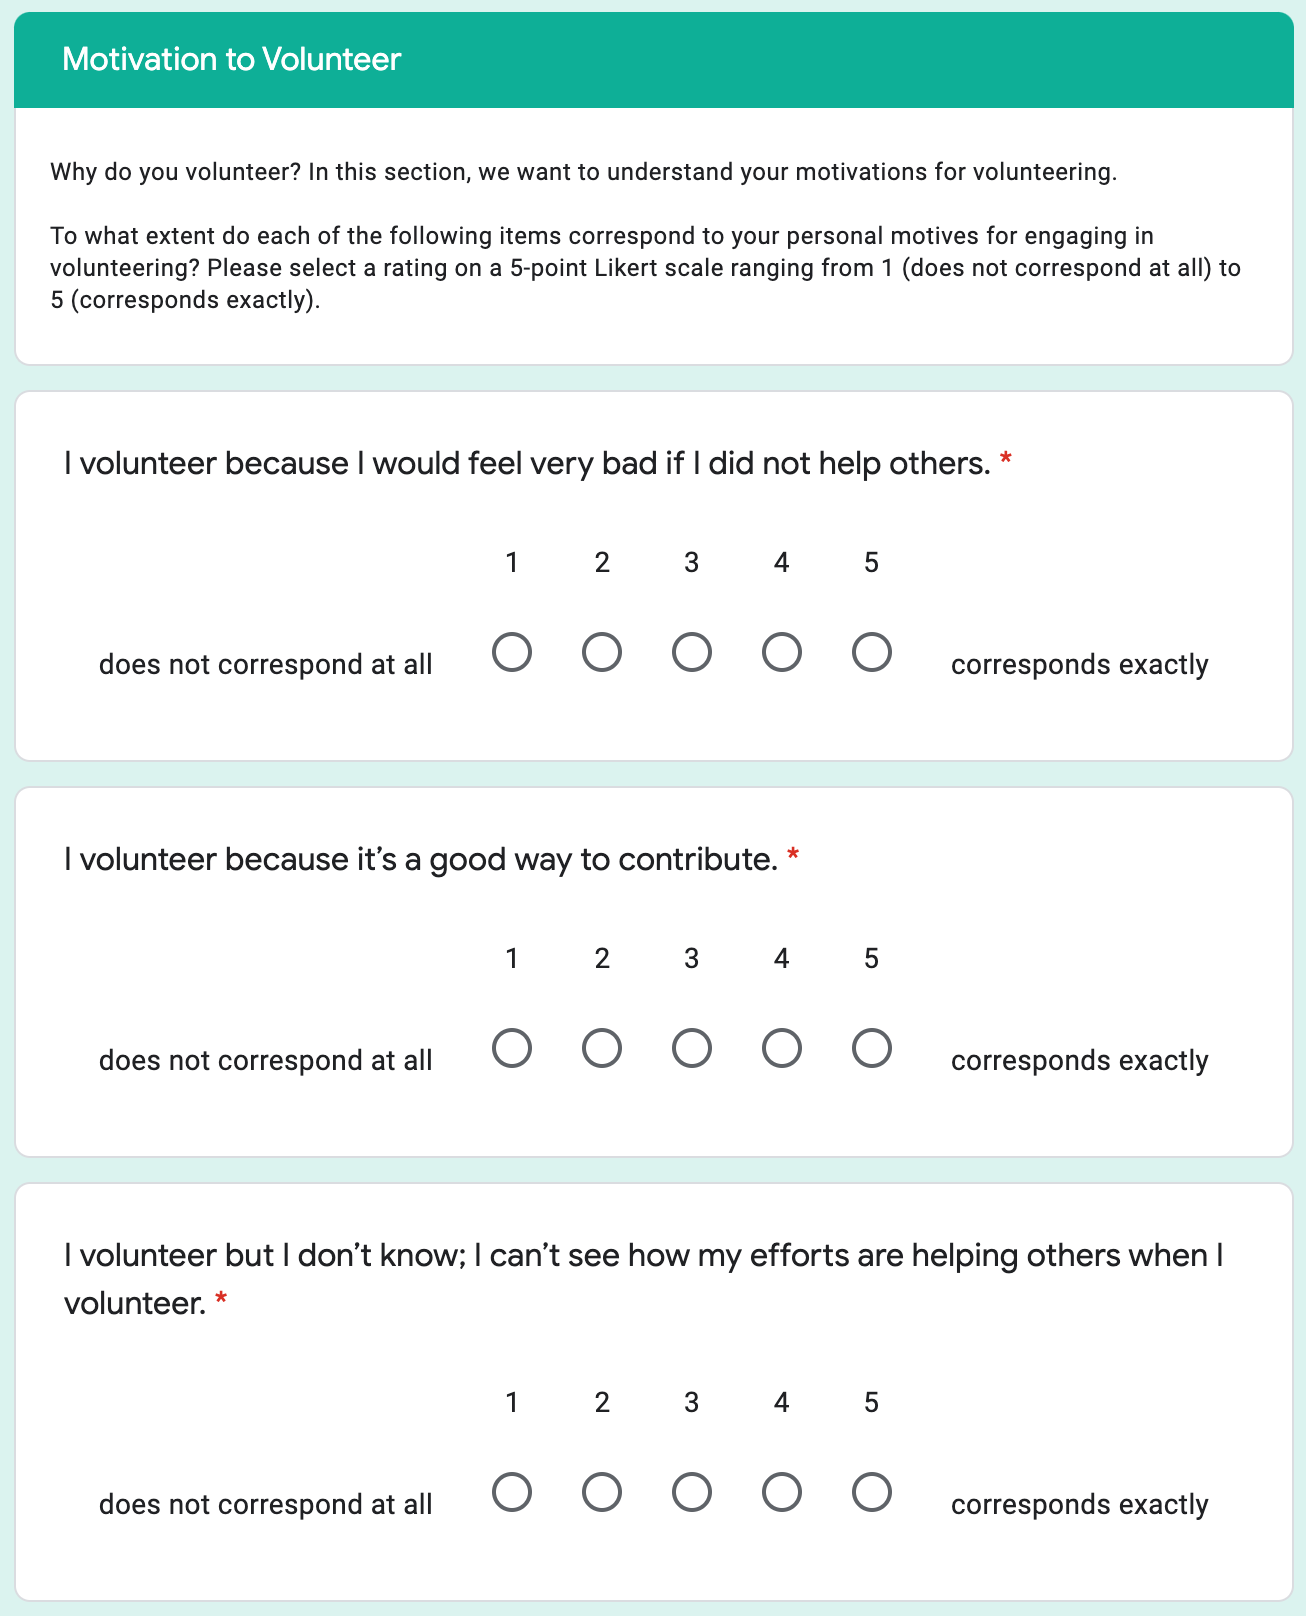
\includegraphics[scale=0.6]{figures/d-mvs.png}
\end{figure}

\begin{enumerate}
    \item I volunteer because I would feel very bad if I did not help others. (\textit{Introjected})
    \item I volunteer because it's a good way to contribute. (\textit{Identified})
    \item I volunteer but I don't know; I can't see how my efforts are helping others when I volunteer. (\textit{Amotivation})
    \item I volunteer because I would feel guilty if I did not volunteer. (\textit{Introjected})
    \item I volunteer because other people will be sorry if I didn't do it. (\textit{External})
    \item I volunteer but I don't know; I can't see how all this helps. (\textit{Amotivation})
    \item I volunteer because I would be ashamed if I did not volunteer. (\textit{Introjected})
    \item I volunteer because it is one of the ways I live my life. (\textit{Integrated})
    \item I volunteer for the pleasure I feel in doing something new. (\textit{Intrinsic})
    \item I volunteer because it's something that contributes to my personal growth. (\textit{Identified})
    \item I volunteer for the pleasure I feel when I master the situations I'm dealing with. (\textit{Intrinsic})
    \item I volunteer because this activity has become an integral part of my life. (\textit{Integrated})
    \item I volunteer for the recognition I get from others. (\textit{External})
    \item I volunteer because volunteering has become a part of who I am. (\textit{Integrated})
    \item I volunteer for the pleasure I feel in finding new ways of help. (\textit{Intrinsic})
    \item I volunteer because it's something that is fulfilling for me as a person. (\textit{Identified})
    \item I volunteer because volunteering is a suitable activity for me. (\textit{Integrated})
    \item I volunteer to avoid being criticized. (\textit{External})
    \item I volunteer but I don't know; I can't see what I’m getting out of it. (\textit{Amotivation})
    \item To show that you are still concentrated, please select 5 for this question. (\textit{Attention Check})
    \item I volunteer because I would regret not doing volunteering. (\textit{Introjected})
    \item I volunteer because I know others are pleased that I volunteer. (\textit{External})
    \item I volunteer for the pleasure and interest I feel in doing this activity. (\textit{Intrinsic})
    \item I volunteer but I don't know; Sometimes I have the impression I'm wasting time when I volunteer. (\textit{Amotivation})
    \item I volunteer because it is a wise thing to do. (\textit{Identified})
\end{enumerate}

The survey also asked how often they participated in volunteering activities in the past three months on average. It was answerable with ``Never,'' ``Once a week,'' and ``Twice a week or more.'' Because the study was conducted during the COVID-19 pandemic and more people tended to volunteer in a crisis, participants were also asked about their average volunteering frequency before the pandemic (October to December 2019).